\subsection{Two electrons in two dimensions}

First, I looked at the simple case of two electrons in a harmonic oscillator trap. These electrons do not interact with each other and the trial wave function is given by Eq. \ref{eq:trial_wf_not_interacing}. 

\subsubsection{Brute force sampling}

Initially, brute force sampling was used to calculate the new position and evaluate the metropolis ratio. The double derivative of the wave function, used to calculate the kinetic energy part of the expectation energy, was evaluated both analytically and numerically to make a comparison. Table \ref{tab:brute_force_no_interaction_2p} shows the energy for different values for the parameter $\alpha$. The numbers show that the standard error of the mean (SEM) is smaller compared to the estimate of the error from the blocking resampling method, $\sigma_B$. This implies that including the correlations, i.e. mainly correlations between one observation and the next where only one particle is moved, increases the estimate of the error. Considering the correlation between the observations gives a more correct estimate of the error, but one has to remember that the deviation from the blocking method only estimate the correlation aspects.

From Tab. \ref{tab:brute_force_no_interaction_2p} one can also observe that $\alpha $ = 1.0 gives zero standard deviation and is therefore the optimal parameter. By comparing the results for the analytical and the numerical cases one can notice that the SEM and $\sigma_B$ is similar for both cases, especially around the ground state ($\alpha$ = 1.0). If the expectation energies from the analytical case and the numerical cases are compared, they differ with values at the scale of $10^{-3}$, which is reasonable with a $\sigma_B$ around $10^{-3}$ to $10^{-2}$. At last one can observe, both from the individual CPU time measurements and the mean CPU time of these 10 measurements (though with different $\alpha$s), that the analytical solution of the double derivative is much faster and more efficient than the numerical case. 

\begin{table}[H]\caption{Comparing the results for analytical/numerical evaluation of the double derivative. Here $\left< E_L \right>$ is the expectation value for the energy given in atomic units (a.u.) and CPU time is in units of seconds. $\sigma_B$ is the standard deviation after resampling with the blocking method and SEM is the standard deviation of the mean. Number of MC cycles are 2$^{21}$.}\label{tab:brute_force_no_interaction_2p}
\center
\begin{tabular}{l|l}
Analytical: &  Numerical:\\ \hline
\begin{tabular}{ccccc}
$\alpha$: & $\left< E_L \right>$: & SEM: & $\sigma_B$: & CPU time:\\ \hline
0.50 & 2.49402 & 0.00073 & 0.01022 & 5.57812\\
0.60 & 2.26441 & 0.00052 & 0.00690 & 5.76562\\
0.70 & 2.13118 & 0.00035 & 0.00448 & 5.92188\\
0.80 & 2.05016 & 0.00022 & 0.00263 & 5.67188\\
0.90 & 2.01015 & 0.00010 & 0.00116 & 5.96875\\
1.00 & 2.00000 & 0.00000 & 0.00000 & 5.62500\\
1.10 & 2.00871 & 0.00009 & 0.00102 & 6.20312\\
1.20 & 2.03402 & 0.00018 & 0.00175 & 6.34375\\
1.30 & 2.07259 & 0.00026 & 0.00244 & 5.95312\\
1.40 & 2.11041 & 0.00034 & 0.00311 & 6.15625\\ \hline
\end{tabular} & \begin{tabular}{ccccc}
$\alpha$: & $\left< E_L \right>$: & SEM: & $\sigma_B$: & CPU time:\\ \hline
0.50 & 2.49991 & 0.00073 & 0.01093 & 18.20310\\
0.60 & 2.26412 & 0.00053 & 0.00727 & 18.21880\\
0.70 & 2.13039 & 0.00036 & 0.00436 & 18.62500\\
0.80 & 2.04993 & 0.00022 & 0.00269 & 18.46880\\
0.90 & 2.01160 & 0.00010 & 0.00118 & 18.46880\\
1.00 & 2.00000 & 0.00000 & 0.00000 & 18.31250\\
1.10 & 2.00825 & 0.00009 & 0.00097 & 18.35940\\
1.20 & 2.03308 & 0.00018 & 0.00170 & 18.31250\\
1.30 & 2.06460 & 0.00026 & 0.00243 & 20.23440\\
1.40 & 2.11803 & 0.00033 & 0.00308 & 19.00000\\ \hline
\end{tabular}\\
Mean CPU time: 5.91875 & Mean CPU time:  18.62033\\
\end{tabular}
\end{table}

\subsubsection{Including importance sampling}

Figure \ref{fig:comparing_sampling} compares the expectation value of the energy and the acceptance rate of brute force sampling and importance sampling. It can be observed from the right part of the figure that the acceptance rate of both methods increase with decreasing step size. These observations could indicate that a small step size would be ideal for both methods. Another observation is that even though the acceptance rate is increasing with smaller step sizes which is a good thing, $\sigma_B$ is also increasing with the step size for both sampling methods  which is not a good thing if $\sigma_B$ is a good estimate of the true error. It could be that this is a balance between number of MC cycles and step size. That, with a smaller step size, one needs a larger number of MC cycles to move the particles enough around to get a true picture of the system, and hence decrease the error.

Furthermore, from the left part of the figure it can be observed that two of the expectation values for the energies are lower than the ground state energy ($dl = 0.005$ and $dl = 0.01$ with brute force sampling) even though these calculations where done with $\alpha$ = 0.9. This should not be possible because the minimum in energy occur for the exact ground state wave function which has $\alpha=1.0$. In addition, in Tab. \ref{tab:compare_stepsize_no_interaction_2p} which compare the result of brute force sampling and importance sampling for different step sizes, one can observe that $\sigma_B$ is larger for the case of brute force sampling with a step size of 0.005 and 0.01. However,  the SEM is smaller at least for $dl = 0.005$ compared to the larger step sizes with brute force sampling and the same step sizes with importance sampling. 

\begin{figure}[H]
\center
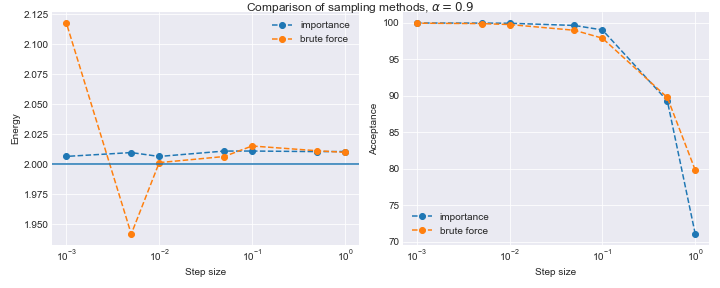
\includegraphics[width=0.85\linewidth]{../Results/comparing_sampling}\caption{Left: Expectation energies after $2^{21}$ MC cycles for different step sizes. Right: Percentage of accepted steps for different step sizes. Here importance sampling and brute force sampling is compared. }\label{fig:comparing_sampling}
\end{figure}


\begin{table}[H]\caption{Comparing the results for importance/brute force sampling. Here the parameter $\alpha$ is set to 0.9 and number of MC cycles are 2$^{21}$. Acc. is short for acceptance and is here given in \% and $t_{CPU}$ is the CPU time used by the program in units of seconds. The rest of the values are as described in Tab. \ref{tab:brute_force_no_interaction_2p}. }\label{tab:compare_stepsize_no_interaction_2p}
\begin{tabular}{l|l|l} 
 & Brute force: &  Importance:\\ \hline
\begin{tabular}{c} 
$dl$:\\ \hline
1.000\\
0.500\\
0.100\\
0.050\\
0.010\\
0.005\\
0.001\\
\end{tabular} & \begin{tabular}{ccccc}
 $\left< E_L \right>$: & SEM: & $\sigma_B$: & Acc.: & $t_{CPU}$:\\ \hline
2.011 & 0.00010 & 0.00067 & 79.794& 7.953\\
2.013 & 0.00010 & 0.00113 & 89.762& 7.719\\
2.019 & 0.00011 & 0.00540 & 97.911& 7.438\\
2.012 & 0.00010 & 0.00801 & 98.980& 7.922\\
1.992 & 0.00010 & 0.02282 & 99.809& 8.141\\
1.920 & 0.00004 & 0.01082 & 99.922& 7.672\\
2.040 & 0.00003 & 0.01043 & 99.976& 7.516\\ \hline
\end{tabular} & \begin{tabular}{ccccc}
$\left< E_L \right>$: & SEM: & $\sigma_B$: & Acc.: & $t_{CPU}$:\\ \hline
2.011 & 0.00010 & 0.00022 & 71.078& 8.531\\
2.011 & 0.00010 & 0.00023 & 89.343& 8.672\\
2.011 & 0.00010 & 0.00047 & 99.049& 8.859\\
2.011 & 0.00010 & 0.00068 & 99.662& 8.188\\
2.007 & 0.00010 & 0.00136 & 99.968& 8.281\\
2.010 & 0.00010 & 0.00199 & 99.989& 8.547\\
2.007 & 0.00010 & 0.00410 & 99.999& 8.016\\ \hline
\end{tabular}\\
& Mean CPU time: 7.766 & Mean CPU time: 8.442 \\
\end{tabular}
\end{table}

I took a closer look at the actual local energies for the brute force sampling method to investigate the cases that gave $\left< E_L \right> < 2.0$. Figure \ref{fig:local_energy_step_size_brute_force} shows that the energy is not stable for steps sizes smaller than 0.01, so even though the step size 0.001 seems to give reasonable expectation values for the energy (see Tab. \ref{tab:compare_stepsize_no_interaction_2p} and Fig. \ref{fig:comparing_sampling}), Fig. \ref{fig:local_energy_step_size_brute_force} shows that it is a lucky shot. I also saw that it was a lucky shot by running the calculation with brute force sampling and the step size, $0.005$, with different seeds for the random number generator. The expectation energy for five different runs where $\left< E_L \right>$ =  1.91487, 2.03452, 1.90805, 1.88356 and 1.9284. From Fig. \ref{fig:local_energy_step_size_brute_force} one can observe that even $dl=0.1$ seems to be too small since it also results in the local energy varying slowly and taking longer "trips" to higher energies and using many steps to get back down again, but for this step size the "trips" to higher energies are more frequent than for the smaller step sizes. I concluded that a step size of 0.5 is the best choice for the brute force sampling because it gives reasonable changes of the local energy and an acceptance rate of $\sim$ 90 \% (see Fig. \ref{fig:comparing_sampling}). 

\begin{figure}[H]
\center
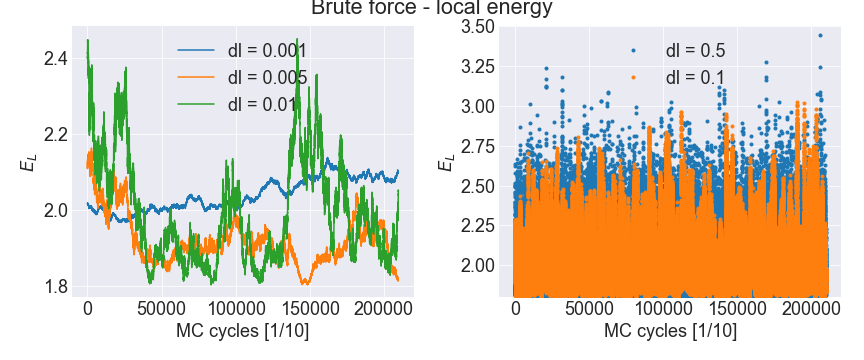
\includegraphics[width=0.85\linewidth]{../Results/local_energy_step_sizes}\caption{The local energy for every tenth MC cycle for brute force sampling at different step sizes, $dl$. a) shows the smaller step sizes and b) some that are a bit larger.}\label{fig:local_energy_step_size_brute_force}
\end{figure}

%On the other hand, for the importance sampling, the investigation of the local energies did not give any clues to why the expecation energy is lower that the ground state energy for a step size of 0.5. Eventually I decided that the result itself indicate that 0.5 is a too large step size for importance sampling and taken together with a low acceptance rate at 0.5 ($\sim$ 82 \%) it is clear that a smaller step size is preferable. 
%
%At last, it is interesting to note that the CPU time of importance sampling is higher than the brute force sampling, so even though brute force sampling has a lower acceptance rate, at the ideal step size, than importance sampling the two methods seems to be somewhat comparable at least for the system I am investigating.

Proceeding to evaluate the energy, Table \ref{tab:ground_state_energy_different_omegas_no_interaction_2p} shows how the energy changes with different trap frequencies, $\omega$.  The energy in the ground state for two electrons is given by 2$\omega$ and this is also the case in Tab. \ref{tab:ground_state_energy_different_omegas_no_interaction_2p}. The table also shows that the kinetic and potential energy follow the virial theorem, i.e. they are equal. They only differ by approximately $\pm 10^{-2} $ $E_h$.


From Tab. \ref{tab:ground_state_energy_different_omegas_no_interaction_2p} one can observe that the mean distance is increasing with decreasing trap frequency.  This is as expected from Fig. \ref{fig:harmonic_oscillator_potential}, where the potential is broadened with decreasing trap frequency and hence is not forcing the particles closer together to the same degree. The mean distance is a bit different for brute force sampling compared to importance sampling, but the similarity might improve if more MC cycles are used. The other value show, however, no large difference between the results from brute force sampling and importance sampling. But to be able to compare the sampling methods more thoroughly it is better to look at the case where the system is not in the ground state. 

\begin{table}[H]\caption{Ground state energy of two electrons in a harmonic oscillator trap.  Here $\overline{r}_{12}$ is the mean distance between the two electrons at positions $\bm{r}_1$ and $\bm{r}_2$ given in units of $a_0$ and $\left< E_L \right>$, $\left< T \right>$, $\left< V_{ext}\right>$  and $\left<V_{int} \right>$ are the expectation value of the local energy, kinetic energy, potential energy and interaction energy, respectively, given in units of $E_h$. The rest of the values are as explained in Tab. \ref{tab:brute_force_no_interaction_2p}. Number of MC cycles are $2^{23}$.}\label{tab:ground_state_energy_different_omegas_no_interaction_2p}
\begin{tabular}{l|l|l} 
 & Brute force: &  Importance:\\ \hline
\begin{tabular}{c} 
$\omega$  \\ \hline
1.00  \\
0.50  \\
0.10  \\
0.05  \\
0.01  \\
\end{tabular} & \begin{tabular}{ccccc}
$\alpha$ & $\left< E_L \right>$ & $\overline{r}_{12} $ & $\left< T \right>$  & $\left< V_{ext}\right>$ \\ \hline
1 & 2.00 & 1.250 & 1.0008 & 0.9992\\
1 & 1.00 & 1.775 & 0.4971 & 0.5029\\
1 & 0.20 & 3.967 & 0.0996 & 0.1004\\ 
1 & 0.10 & 5.638 & 0.0497 & 0.0503\\ 
1 & 0.02 & 12.631 & 0.0099 & 0.0101\\  
\end{tabular} & \begin{tabular}{ccccc}
$\alpha$ & $\left< E_L \right>$ & $\overline{r}_{12} $ & $\left< T \right>$  & $\left< V_{ext}\right>$ \\ \hline
1 & 2.00 & 1.254 & 0.9982 & 1.0018\\
1 & 1.00 & 1.781 & 0.4973 & 0.5027\\
1 & 0.20 & 4.046 & 0.0987 & 0.1013\\ 
1 & 0.10 & 5.534 & 0.0512 & 0.0488\\ 
1 & 0.02 & 12.488 & 0.0101 & 0.0099\\ 
\end{tabular}\\
\end{tabular}
\end{table}

Table \ref{tab:compare_importance_alphas_2p} shows the expectation value of the energy for various parameters, $\alpha$.  The calculated expectation values for the energy for the two different sampling methods are similar, especially close to the correct parameter $\alpha$, varying only by $\pm 10^{-2}$. However, what is different is that $\sigma_B$ is larger for importance sampling than for brute force sampling. I do not know why there is a difference there. Maybe the estimate of the error is more correct, but the blocking code is the same, hence it would have to be that the sampling results in a different correlation. On the other hand, it could be that there is a larger error when using importance sampling. But it could also be that I should have chosen a larger step size for importance sampling since $\sigma_B$ increased with the decrease of the step size. 

At last, one can observe that the CPU time of the importance sampling method is larger than brute force sampling which is as expected because of the calculation of the gradient in the quantum force. But we know from Fig. \ref{fig:comparing_sampling} that the acceptance rate of brute force sampling is around 90 \% compared to importance sampling which should be close to 100 \% and this makes the importance sampling technique more effective in terms of MC cycles.

\begin{table}[H]\caption{Comparing the results for brute force sampling/importance sampling. Values are as explained in Tab. \ref{tab:brute_force_no_interaction_2p}. Number of MC cycles are 2$^{21}$.}\label{tab:compare_importance_alphas_2p}
\center
\begin{tabular}{l|l|l}
 & Brute force: & Importance:\\ \hline
\begin{tabular}{c}
$\alpha$: \\ \hline
0.50 \\
0.60 \\
0.70 \\
0.80 \\
0.90\\
1.00 \\
1.10 \\
1.20 \\
1.30\\
1.40 \\ \hline
\end{tabular} & \begin{tabular}{cccc}
 $\left< E_L \right>$: & SEM: & $\sigma_B$: & CPU time:\\ \hline
2.49074 & 0.00072 & 0.01030 & 6.26562\\
2.27645 & 0.00053 & 0.00721 & 6.53125\\
2.12481 & 0.00036 & 0.00451 & 6.59375\\
2.04873 & 0.00022 & 0.00265 & 6.68750\\
2.01135 & 0.00010 & 0.00115 & 6.82812\\
2.00000 & 0.00000 & 0.00000 & 6.75000\\
2.00863 & 0.00009 & 0.00097 & 6.59375\\
2.03343 & 0.00018 & 0.00174 & 7.29688\\
2.07103 & 0.00026 & 0.00246 & 6.75000\\
2.11725 & 0.00033 & 0.00317 & 6.70312\\ \hline
\end{tabular} & \begin{tabular}{cccc}
$\left< E_L \right>$: & SEM: & $\sigma_B$: & CPU time:\\ \hline
2.52950 & 0.00075 & 0.01952 & 8.53125\\
2.26531 & 0.00052 & 0.01281 & 8.62500\\
2.12449 & 0.00036 & 0.00813 & 8.76562\\
2.04797 & 0.00022 & 0.00454 & 9.37500\\
2.01171 & 0.00010 & 0.00203 & 8.81250\\
2.00000 & 0.00000 & 0.00000 & 8.76562\\
2.00954 & 0.00009 & 0.00171 & 8.40625\\
2.03276 & 0.00018 & 0.00305 & 8.50000\\
2.07363 & 0.00026 & 0.00440 & 8.67188\\
2.10697 & 0.00034 & 0.00536 & 8.67188\\ \hline
\end{tabular}\\
& Mean CPU time:  6.7000 & Mean CPU time:  8.7125\\
\end{tabular}
\end{table}


\subsubsection{Including optimization}

In this project there are two parameters to optimize and hence it is a more complicated problem. I chose, in this project compared to the previous one, to experiment with the minimization rate during the actual optimization. I anticipated that the ideal minimization rate would be different for the different size systems and therefore an analysis of one system would not transfer to the other systems. I started out using a minimization rate, $\gamma$ = 0.5. It resulted in few steps until the parameter value stabilized both for guesses close to the optimal value and for guesses far away from the optimal value, but for the smallest trap frequencies I had to use $\gamma = $ 0.1 or 0.2. For the case of two interacting fermions, the parameters were optimized by trying out different first guesses for $\alpha$ and $\beta$ and tuning $\gamma$ so that the parameters stabilized during the first 200 iterations. The optimal parameters were extracted from the mean of the last 50 iterations. An example run is shown in Fig. \ref{fig:example_gradient_descent} for $\omega = 0.5$.

\begin{figure}[H]
\center
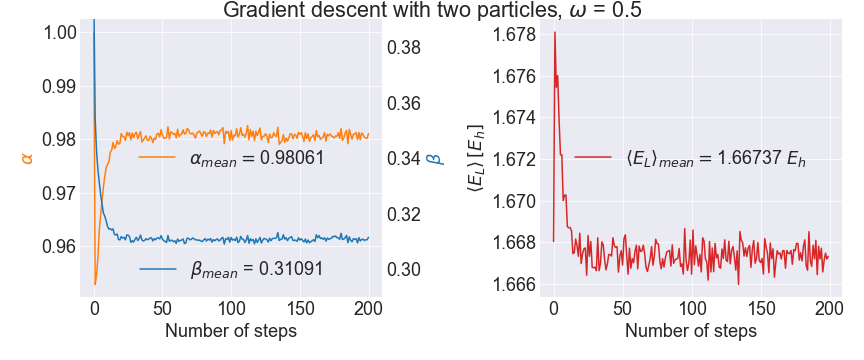
\includegraphics[width=0.8\linewidth]{../Results/example_gradient_descent}\caption{Left: The development of the parameters during the steps of gradient descent. The values $\alpha_{mean}$ and $\beta_{mean}$ printed on the figure is the mean of the last 50 values. Right: The expectation value after $2^{19}$ number of MC cycles. Here also, the value printed on the figure is the mean of the last 50 iterations. }\label{fig:example_gradient_descent}
\end{figure}

For the system with six interacting electrons, the method described above was used for the largest $\omega$s (i.e. $\omega$ = 1.0, 0.5, 0.1), but for the smaller ones I had to use a smaller minimization rate (i.e. 0.01-0.05) and I also had to move step by step from $\omega$ = 0.1 to $\omega$ = 0.01 with the step size of $\Delta \omega = 0.01$. I found the parameters for the current $\omega$ and used that as a guess for the next $\omega$. I tried to do it in a more efficient way and let the simple gradient descent method find the minimum on its own, but with this unguided method, the optimization ended up in local minima at higher energies or going to infinite energies. To improve the code, I attempted to use the extended gradient descent method, described in project 1, which utilize the previous gradient to find the new parameter  \cite{project1}. But the attempt did not improve the behaviour described earlier. Compared to project 1, this system's local energy dependence on the parameters  ($\left< E_L \right> (\alpha, \beta)$), is more complicated, and also involve two parameters instead of one, which makes it harder to optimize the parameters with this simple gradient descent method.

%The right part of Fig. \ref{fig:example_gradient_descent} shows mean of $\left< E_L \right>$ 50 runs with $2^{19}$ MC cycles with slightly different $\alpha$s and $\beta$s (eft part of the same figure), which values are oscillating around the optimal value. This set-up made me wonder is this estimate of the energy is better than performing one calculation with the mean values of $\alpha$ and $\beta$ for the same number of MC cycles, i.e. $50 \cdot 2^{19}$. My thought process was that if the mean value of the $\alpha$ and $\beta$ is not the optimal value, then the varying $\alpha$s and $\beta$s could be a better choice.  

\subsubsection{Including interaction}

Here is the results of the expectation values approximating the ground state energy for two interacting electrons in a harmonic oscillator trap. The equations used to model the system is as described in the theory part of this report. That includes the trial wave function (see Eq. \ref{eq:trial_interacting}) with the Jastrow factor that is used to model the many-body wave function. Table \ref{tab:ground_state_energy_importance_interaction} shows the results of the calculations with the optimal parameters found with the gradient descent method with importance sampling. 

\begin{table}[H]\caption{Ground state energy of two interacting electrons in harmonic oscillator trap found with importance sampling. Here $\overline{r}_{12}$,  $\left< T \right>$, $\left< V_{ext}\right>$  and $\left<V_{int} \right>$as explain in Tab. \ref{tab:ground_state_energy_different_omegas_no_interaction_2p}. The rest of the values are as explained in Tab. \ref{tab:brute_force_no_interaction_2p}. Number of MC cycles are $2^{23}$}\label{tab:ground_state_energy_importance_interaction}
\center
\begin{tabular}{c|ccccccccc}
$\omega$ & $\alpha$ & $\beta$ & $\left< E_L \right>$ & SEM & $\sigma_B$ &  $\overline{r}_{12} \,\,\,$ & $\left< T \right>$  & $\left< V_{ext}\right>$ & $\left<V_{int} \right>$  \\ \hline
1.00 & 0.98846 & 0.39954 & 3.0069 & 0.00001 & 0.00018 & 1.643 & 0.8931 & 1.3052 & 0.8086\\
0.50& 0.98082 & 0.31068 & 1.6674 & 0.00001 & 0.00019 & 2.481 & 0.4547 & 0.6997 & 0.5130\\
0.10 & 0.94734 & 0.17810 & 0.4486 & 0.00001 & 0.00023 & 6.724 & 0.0989 & 0.1787 & 0.1710\\
0.05 & 0.92262 & 0.14090 & 0.2610 & 0.00000 & 0.00021 & 10.333 & 0.0495 & 0.1024 & 0.1091\\
0.01 & 0.88305 & 0.07366 & 0.0776 & 0.00000 & 0.00010 & 29.293 & 0.0131 & 0.0283 & 0.0362\\
\end{tabular}
\end{table}


Table \ref{tab:ground_state_energy_importance_interaction} shows that the expectation energy for the ground state with $\omega = 1.0$ is $3.0069 \pm 0.0002$ $E_h$. This result is not that far away from the exact value of $3$ $E_h$ from Taut's work \cite{taut1993two}. The energy of the system is decreasing with decreasing trap frequency, $\omega$. One can also observe that the potential energy dominates for large trap frequencies ($\omega = 1.0$ and $\omega = 0.5$), but for the smaller $\omega$s the interaction energy and the potential energy is approximately equal.  This seems to be reasonable since the potential energy is sort of stored in the force from the trap. The potential keeps the electrons together which means that a larger trap frequency gives a stronger trapping force and hence a larger potential energy.  For all $\omega$, the kinetic energy is the smallest one and it also decrease with the decreasing trap frequency. This also makes sense because the energy of the individual electron will oscillate between potential energy (either from the external potential or the potential from the interaction) and kinetic energy and when the potential energy decrease, the kinetic energy will decrease with it.

\begin{figure}[H]
\center
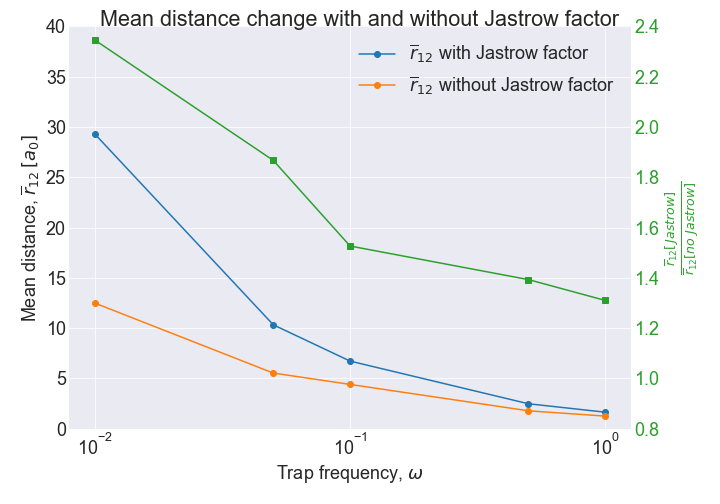
\includegraphics[width=0.7\linewidth]{../Results/mean_distance_change}\caption{The mean distance between the two particles, calculated with importance sampling, compared for the situation with and without the Jastrow factor and at different trap frequencies. }\label{fig:mean_distance_compared}
\end{figure}

Figure \ref{fig:mean_distance_compared} shows the combined results from Tab. \ref{tab:ground_state_energy_different_omegas_no_interaction_2p} and \ref{tab:ground_state_energy_importance_interaction}. One can observe that the mean distance is larger for the case with interaction. This is expected since the interaction potential (see Eq. \ref{eq:hamilton_interaction}) is a repulsive potential, and will hence force the electrons further apart. One can also observe that the ratio of the two different cases (right axis and green color) increase with decreasing trap frequency, i.e. the mean distance increases more for smaller trap frequencies. This could imply that the trap frequency is influencing the mean distance even more than the inclusion of interaction.

\subsubsection{One-body density}

The one-body density tells how the particles are distributed in space, and Fig. \ref{fig:one_body_density_no_interaction_2p} shows the result of the one-body density of the system of two not interacting fermions for different trap frequencies. One can observe, as one saw in the development of the mean distance (see Fig. \ref{fig:mean_distance_compared}), that the particle distribution or density is spread out in space for smaller trap frequencies. From Fig. \ref{fig:one_body_density_no_interaction_2p} one can also observe that the electrons spend most of their time around the origin of the harmonic oscillator trap. The shape of the curve seems not to change for the different trap frequencies, only the height and width.

\begin{figure}[H]
\center
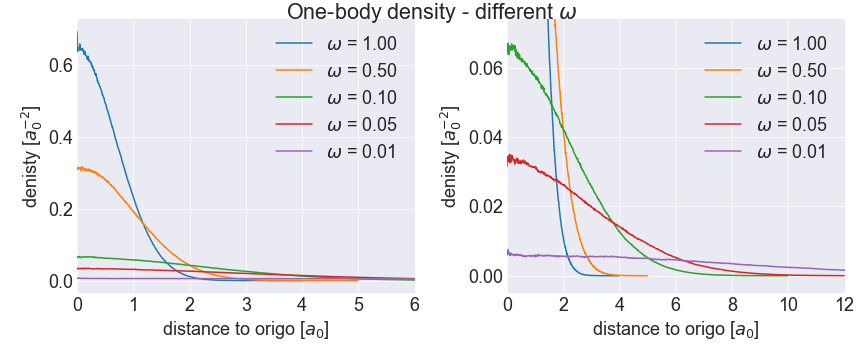
\includegraphics[width=0.85\linewidth]{../Results/one_body_density_no_interaction_2p}\caption{One-body density of the two electron system without the Jastrow factor, but with different trap frequencies. Left: The larger trap frequencies. Right: The smaller trap frequencies. The system with $\omega = 0.1$ is in both plots to show the difference in scale for the two plots. Used $2^{24}$ MC cycles. }\label{fig:one_body_density_no_interaction_2p}
\end{figure}

To get a smooth curve, I found out that you either have to use larger bin sizes or more MC cycles. Since the one-body density is found by counting how many times a particle is situated within a certain bin, i.e. with a certain distance to origin, more samples of the positions will give a more true distribution. So if the bin size is small, you need more MC cycles to smooth out the random difference based on the number of samples between two neighbouring bins. On the other hand, if the bin size is too large real differences or fast changes in the distribution might not be detected.

Furthermore, Fig. \ref{fig:one_body_density_interaction_2p} shows the one-body densities with and without the Jastrow factor. Here, one can also observe the same as was seen with the mean distance, that the Jastrow factor spreads out the distribution of the particles, but the difference is a lot clearer in the one-body density plot. Another interesting observation is that, for the interacting case, the maximum does not seem to lay at the origin. It is not that easy to see for the larger trap frequencies, but one can easily see it for $\omega = 0.1$ in the right part of Fig. \ref{fig:one_body_density_interaction_2p}. This seems to be reasonable because there is a repulsive force between the particles, they spend more time further away from the origin. It could be that for larger trap frequencies there is a larger energy related gain ( i.e. the energy is lower) to be situated closer to origin, hence the maximum is not shifted as far from origin for those frequencies, but for the lower trap frequencies the gain obtained closer to origin does not compensate enough of the repulsive forces (or interaction energy), so the maximum is shifted away from origin. That should imply that the position of the maximum reflects a balance between the potential energy and the interaction energy. 

\begin{figure}[H]
\center
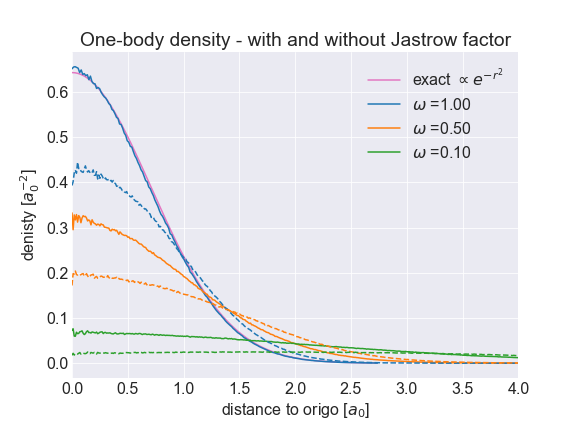
\includegraphics[width=0.85\linewidth]{../Results/one_body_density_interaction_2p}\caption{One-body density of the two electron system with and without the Jastrow factor and with different trap frequencies (indicated by the color of the lines). Dashed lines are with the Jastrow factor and filled lines are without Jastrow factor. Left: The larger trap frequencies. Right: The smaller trap frequencies.  The system with $\omega = 0.1$ is in both plots to show the difference in scale for the two plots. Used $2^{24}$ MC cycles. }\label{fig:one_body_density_interaction_2p}
\end{figure}

\subsection{Six particles}

To investigate the quantum dot system further, the next shell (illustrated in Fig. \ref{fig:states}) is filled and this results in a system of six particles. The expectation value for the total energy (i.e. the local energy), the kinetic energy and the potential energy for the different trap frequencies without interaction are listed in Tab. \ref{tab:ground_state_energy_importance_6p}. One can observe that for all the trap frequencies, the kinetic and potential energy seems to follow the virial theorem (see Eq. \ref{eq:virial_theorem}), if one allows for a small difference of maximum $\pm 0.03$ a.u.. The energies are as expected from the calculated exact energies in Tab.  \ref{tab:exact_energies_non_interacting} in Appendix \ref{app:energies}.

\begin{table}[H]\caption{Ground state energy of six electrons in a harmonic oscillator trap. Here $\left< E_L \right>$, $\left< T \right>$ and $\left< V_{ext}\right>$  are as explain in Tab. \ref{tab:ground_state_energy_different_omegas_no_interaction_2p}. Number of MC cycles are $2^{23}$. }\label{tab:ground_state_energy_importance_6p}
\center
\begin{tabular}{c|rcc}
$\omega$ & $\left< E_L \right>$  & $\left< T \right>$  & $\left< V_{ext}\right>$ \\ \hline
1.00 & 10.00 & 4.9865 & 5.0135\\ 
0.50 & 5.00 & 2.4973 & 2.5027\\
0.10 & 1.00 & 0.4861 & 0.5139\\
0.05 & 0.50 & 0.2483 & 0.2517\\
0.01 & 0.10 & 0.0454 & 0.0546\\
\end{tabular}
\end{table}

Furthermore, the result after including interaction is showed in Tab. \ref{tab:ground_state_energy_importance_interaction_6p}. One can observe, if one compares the result with Tab. \ref{tab:ground_state_energy_importance_interaction}, that the both the SEM and $\sigma_B$ are larger for the system with six electrons. This could be explained by the fact that the total energies are larger for this system, and hence the errors will be larger. If one compare the error as a fraction for the case with $\omega = 1.0$ $\nicefrac{\sigma_B}{\left< E_L \right>} = 5.99 \cdot 10^{-5}$ for two electrons and $3.98\cdot 10^{-4}$ for six electrons and one can see that the error is larger for the six electron case as a fraction as well. This made me wonder if $\sigma_B$ would be worse if the optimal parameters where worse, but $\sigma_B$ indicate how good the expectation value is for the parameters given. It tells if the expectation value that comes out can be relied upon. It does not tell us how far the expectation value is from the real energy.

\begin{table}[H]\caption{Ground state energy of six interacting electrons in harmonic oscillator trap found with importance sampling. Number of MC cycles are $2^{23}$.}\label{tab:ground_state_energy_importance_interaction_6p}
\center
\begin{tabular}{c|cccccccc}
$\omega$ & $\alpha$ & $\beta$ & $\left< E_L \right>$ & SEM & $\sigma_B$ &  $\left< T \right>$  & $\left< V_{ext}\right>$ & $\left<V_{int} \right>$  \\ \hline
1.00 & 0.71567 & 0.49372 & 20.4492 & 0.00022 & 0.00813 & 2.3429 & 10.7076 & 7.3988\\
0.50 & 0.75823 & 0.34260 & 11.9868 & 0.00011 & 0.00522 & 1.3226 & 5.8094 & 4.8548\\
0.10 & 0.78852 & 0.15041 & 3.6542 & 0.00003 & 0.00416 & 0.2951 & 1.7035 & 1.6556\\
0.05 & 0.76518 & 0.10733 & 2.2223 & 0.00003 & 0.00436 &  0.1178 & 1.0882 & 1.0162\\
0.01 & 0.64907 & 0.05085 & 0.7191 & 0.00001 & 0.00586 & 0.0021 & 0.3803 & 0.3367\\
\end{tabular}
\end{table}

I wanted to take a closer look at the optimized parameters for the two different systems too, especially since I had so much trouble finding the parameters for the six electron system. Figure \ref{fig:parameters_compared} compares the optimized parameters for the two systems with different amounts of particles at the different trap frequencies. One can observe that the $\beta$ parameter which is involved in the Jastrow factor is similar for both systems and also show a similar development from one trap frequency to the next. This is expected, I guess, since the interaction between the particles do not change that much by increasing the number of particles. The other parameter $\alpha$, however, which is involved in the Slater determinant, shows completely different values and development for the two systems. This is also reasonable because the wave function, i.e. the Slater determinant part, changes a lot when we increase the number of particles. Because when the number of particles is increased higher states with very different single-particle wave functions are filled and the Slater determinant is changed a lot. The development of $\alpha$ though is strange, I would have expected it to either increase or decrease with an increasing trap frequency, but in the right part of Fig. \ref{fig:parameters_compared} one can observe that the largest $\alpha$ is found for $\omega = 0.1$ which is the middle $\omega$ investigated. But my expectations might be wrong, maybe the strange development is due to the single-particle states that are introduced with the higher energy states. 

\begin{figure}[H]
\center
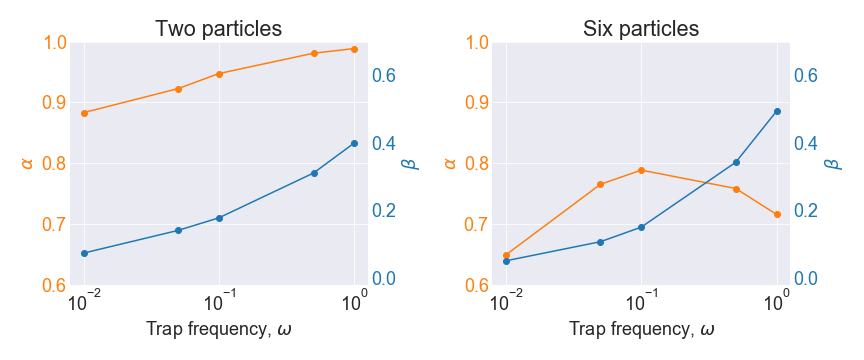
\includegraphics[width=0.85\linewidth]{../Results/parameters_compared}\caption{Left: The optimized parameters for the system with two particles and with the different trap frequencies. Right: The optimized parameters for  for the system with six particles and with the different trap frequencies. All found with the simple gradient descent method.}\label{fig:parameters_compared}
\end{figure}

Next, Fig. \ref{fig:energy_per_particle_compared} compares the energy per particle of the two systems when interaction is included. The left part of the figure shows that the magnitude of kinetic energy per particle and the development of the kinetic energy with trap frequency is very similar for both systems (two and six particles). The right part of the figure shows that both the potential and interaction energy per particle is larger for the six particle system at the same trap frequency, than the two particle system. This is as expected since the trap frequency determine the "size" of the trap. The six particle system's potential energy is hence larger for the same size system when there are more particles involved. The interaction energy is also larger when more particles, that are repulsed by each other, are forced together in the "same amount of space" (it is not exactly the same amount of space since the space is not strictly limited, but it is intuitive to image it like that). Apart from this, the six particle system show the same behaviour as the two particle system, with regards to energy. 

\begin{figure}[H]
\center
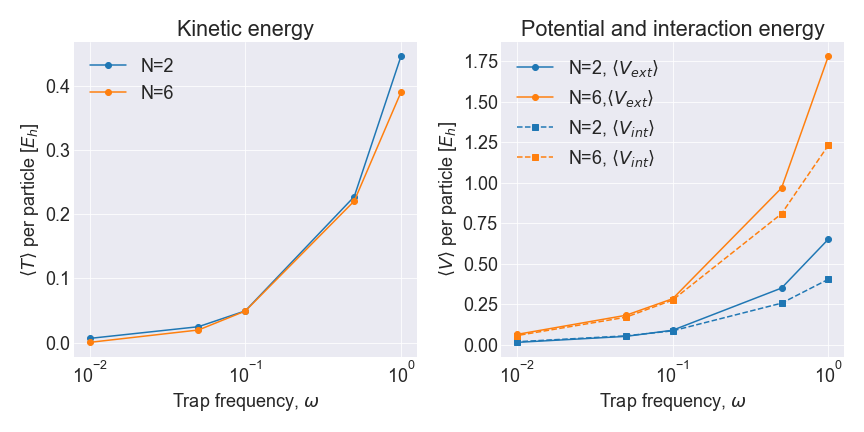
\includegraphics[width=0.85\linewidth]{../Results/energy_per_particle_compared}\caption{Left: The expectation value for the kinetic energy per particle for the two different systems examined at the different trap frequencies. Right: The expectation value of the potential and interaction energy per particle for the two different systems at the different trap frequencies.  }\label{fig:energy_per_particle_compared}
\end{figure}

Proceeding to the one-body density, Fig. \ref{fig:one_body_density_interaction_6p} shows the one-body density for the six electron system. First, one can notice that the shape is different from the two electron system. Here the maximum density is not at the origin of the trap, but approximately $a_0$ away from the origin for $\omega=1.0$ without the Jastrow factor. Furthermore, one can observe that the maximum moves further and further away from the origin when $\omega$ increases. Regarding the inclusion of interaction, the same behaviour is seen here, compared to the two electron one-body density, that including interaction  broadens the whole curve and lowers the maximum density. The shape of the one-body density curve seems to be similar with and without interaction except for $\omega = 0.1$ and maybe also smaller $\omega$ where there is another maximum closer to the origin. Maybe the broadening of the trap with decreasing $\omega$ opens up for a redistribution of the particles when the repulsive interaction is included. 

\begin{figure}[H]
\center
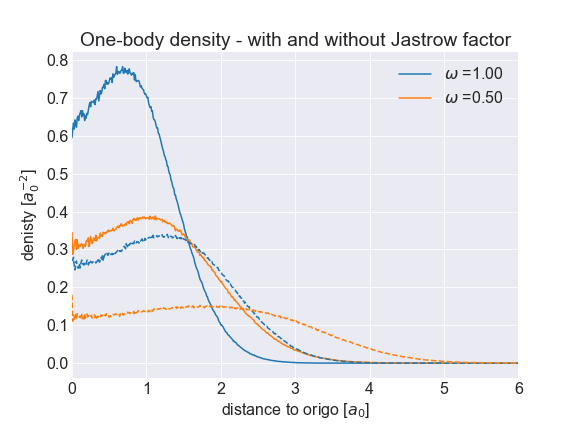
\includegraphics[width=0.85\linewidth]{../Results/one_body_density_interaction_6p}\caption{One-body density of the six electron system with and without the Jastrow factor and with different trap frequencies (indicated by the color of the lines). Dashed lines are with the Jastrow factor and filled lines are without Jastrow factor. Left: The larger trap frequencies. Right: The smaller trap frequencies.  The system with $\omega = 0.1$ is in both plots to show the difference in scale for the two plots. Used $2^{24}$ MC cycles. }\label{fig:one_body_density_interaction_6p}
\end{figure}


\subsection{Twelve particles}

By including another shell in the two dimensional harmonic oscillator trap, the system consists of twelve particles. The ground state energy at different $\omega$s are listed in Tab. \ref{tab:ground_state_energy_importance_12p} and the energies are the same as the exact energies calculated from the energy of the different states (see Tab. \ref{tab:exact_energies_non_interacting} in Appendix \ref{app:energies}).

\begin{table}[H]\caption{Ground state energy of twelve electrons in a harmonic oscillator trap. Here $\left< E_L \right>$, $\left< T \right>$ and $\left< V_{ext}\right>$  are as explain in Tab. \ref{tab:ground_state_energy_different_omegas_no_interaction_2p}. Number of MC cycles are $2^{23}$. }\label{tab:ground_state_energy_importance_12p}
\center
\begin{tabular}{c|rrr}
$\omega$ & $\left< E_L \right>$  & $\left< T \right>\,\,\,$  & $\left< V_{ext}\right>\,$ \\ \hline
1.00 & 28.00 & 14.0117 & 13.9883\\ 
0.50 & 14.00 & 7.0463 & 6.9537\\ 
0.10 & 2.80 & 1.4084 & 1.3916\\ 
0.05 & 1.40 & 0.6901 & 0.7099\\ 
0.01 & 0.28 & 0.1419 & 0.1381\\ 
\end{tabular}
\end{table}

I tried to use the same method, the simple gradient descent method, to evaluate the parameters that gives me the closest thing to the ground state I can get with the trial wave function used in this project, but it seems like the system got too complicated with twelve particles. An example of the behaviour of the gradient descent method is showed in Fig. \ref{fig:gradient_descent_12p}. One can observe, from the right part of the figure that the energy seems to be converging towards a minimum, but it is a very slow process. However, the left part of the figure shows how much the parameters are varying and that the parameter $\alpha$ is negative. I do not think that a negative $\alpha$ is a good sign especially after comparing my results with Ref. \cite{Evens_master} where $\left< E_L \right> = 65.7026(4)$ was found for the same system. It is strange that I get an energy that much smaller than the energy calculated in Ref. \cite{Evens_master} considering that all wave functions except the ground state wave function should give larger energies than the ground state energy. However, the negative $\alpha$ could be the explanation if it makes the wave function not physical.

\begin{figure}[H]
\center
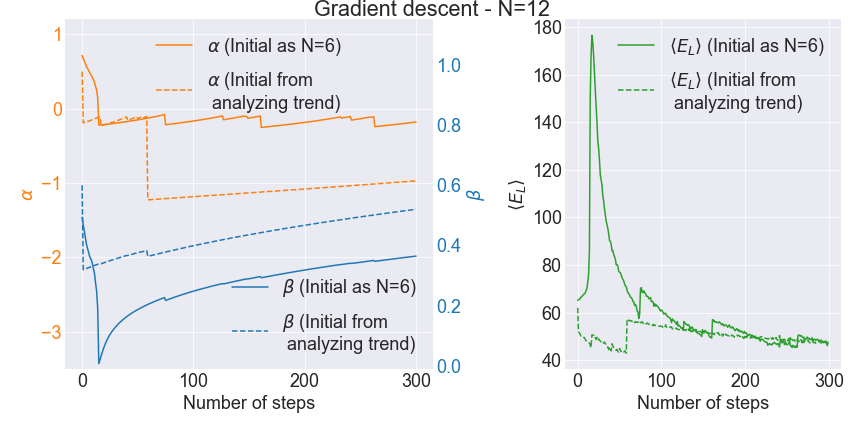
\includegraphics[width=0.85\linewidth]{../Results/gradient_descent_12p}\caption{Two examples of the gradient descent method for twelve particles with different initial guesses for the two parameters. One of them is a guess based on the parameters found for the six electron system and the other is a guess based on the difference and trend found when the two electron and the six electron parameters was compared. Left: The development of the parameters. Right: The corresponding expectation value for the energy. }\label{fig:gradient_descent_12p}
\end{figure}

Continuing to the one-body density, Fig. \ref{fig:one_body_density_no_interaction_12p} shows the one-body density for the twelve electron system, but only without interaction since a ground state for the interacting system was not found. Compared to the two smaller systems, this system shows another curve for the one-body density. Here, the maximum is once again at the origin of the trap, but there is also another local maximum approximately 1.5$a_0$ away from the origin for $\omega = 1.0$. The scaling of the density seems to be similar to the former two systems where one see that the distribution broadens and the maximum is hence lowered, but the shape remains similar when $\omega$ is decreased.

\begin{figure}[H]
\center
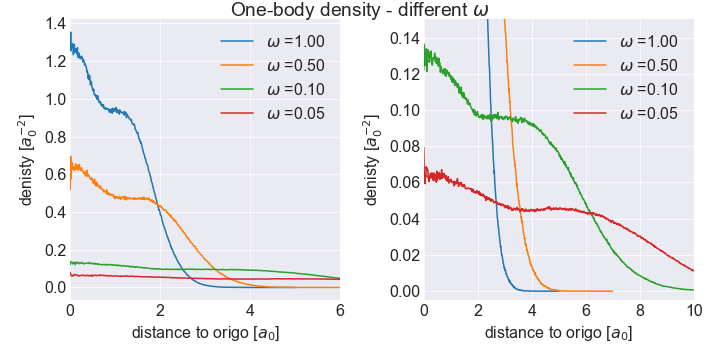
\includegraphics[width=0.85\linewidth]{../Results/one_body_density_no_interaction_12p}\caption{One-body density of the twelve electron system without the Jastrow factor, but with different trap frequencies. Left: The larger trap frequencies. Right: The smaller trap frequencies. The system with $\omega = 0.1$ is in both plots to show the difference in scale for the two plots. Used $2^{24}$ MC cycles. }\label{fig:one_body_density_no_interaction_12p}
\end{figure}

\subsection{Efficiency}

In this project I wanted to write an efficient code, but I ran into some problems and after a while I figured out that it was best to use the not so efficient, but working code to get some results and use time to analyse them. Therefore, I have two branches in my repository at \href{https://github.com/vildemjo/vmc_fermions}{GitHub}. One called \texttt{no\_optimization} and one master branch. The master branch includes my attempts to make the code more efficient as described in the theory part of this report, and the other branch is the code used to generate the results in this project. Both branches do include an efficient way of calculating the gradient and the double derivative though.

\subsection{Performance analysis}

At last, I include a small analysis of the performance of the code with and without vectorization and with and without parallelizing.

\subsubsection{Vectorization}

Table \ref{tab:CPUtime_vectorization} lists the average CPU time of ten runs of the code with and without vectorization. The mean was found four times for both cases at different times during a working day. There is not a clear difference in CPU time, and one can also see from the four different attempts, that the CPU time changes based on the computer. I think one can conclude that the program is just as efficient with and without the vectorization. But this is just comparing the CPU time. As I have understood, vectorization can also help exploit the computer memory in a more efficient way. 

\begin{table}[H]\caption{The average CPU time in seconds after 10 runs. The calculation is of the six electron system with interaction and involves importance sampling, saving and printing all local energies to file. Here I used $2^{22}$ MC cycles. }\label{tab:CPUtime_vectorization}
\center
\begin{tabular}{c|cc}
 & CPU time & \\ \hline
Run & With vectorization & Without vectorization \\ \hline
1 & 145.930 & 148.531 \\
2 & 149.653 & 142.881 \\
3 & 155.731 & 153.519 \\
4 & 146.769 & 146.834 \\
\end{tabular}
\end{table}

\subsubsection{Parallellization}

The CPU times for the different threads for five different runs are listed in Tab. \ref{tab:CPUtime_treads}. The maximum CPU time of the four different threads is counted as the total CPU time. From the different runs, one can observe that the CPU time can vary based on the laptop and other processes on it, and it shows that it is important to time several runs to get a proper comparison of the CPU time of different methods. 

\begin{table}[H]\caption{Four threads $2^{22}$ MC cycles on each.}\label{tab:CPUtime_treads}
\center
\begin{tabular}{r|cccc|c}
Thread & 1 & 2 & 3 & 4 & Total: \\ \hline
CPU time & 206.520 & 207.370 & 209.260 & 210.400 & 210.400 \\
& 228.270 & 229.930 & 229.930 & 230.110 & 230.110 \\
& 231.880 & 234.690 & 235.030 & 235.730 & 235.730 \\
& 231.330 & 234.060 & 234.170 & 234.300 & 234.300 \\
& 230.200 & 231.280 & 231.770 & 232.070 & 232.070 \\ \hline
 &  &  &  & Mean: & 228.522 \\
\end{tabular}\\
\end{table}

Table \ref{tab:CPUtime_parallelization} compare the CPU time of parallelized runs and the not parallelized runs. One can see clearly that the parallelized runs are faster, but even though the parellelized run is done on four threads it is only between two and three times faster. One reason might be that the number of MC cycles used to reach an equilibrium is the same ($1\cdot 10^5$) for both cases. For the single thread case it is done only once and afterwards all the local energies are sampled, but for the four thread case this is done independently on all four threads.

\begin{table}[H]\caption{Not parallelized: $2^{24}$ MC cycles and one thread. Parallelized: $2^{22}$ MC cycles and four threads. The CPU times are given in seconds and as an average over five runs.}\label{tab:CPUtime_parallelization}
\center
\begin{tabular}{r|ccc}
& Not parallelized & Parallelized & Times faster \\ \hline
CPU time &  656.210  & 228.522 & 2.87\\
 & 602.816   & 257.922  & 2.34\\
\end{tabular}
\end{table}

At last I compared the expectation value, the SEM and $\sigma_B$ for one of the runs with and without parallelizing. The results are listed in Tab. \ref{tab:energy_parallelization} and shows a difference in the expectation value of the energy at approximately $\pm 0.01$ which is larger than the calculated $\sigma_B$. One would expect a difference because of the different seeds in the random number generator, but maybe not that large. This might improve with a larger number of MC cycles though. 

\begin{table}[H]\caption{A comparison of the expectation value, the SEM and $\sigma_B$ for one of the runs with and without parallelizing. Units are as described in Tab. \ref{tab:ground_state_energy_different_omegas_no_interaction_2p}.}\label{tab:energy_parallelization}
\center
\begin{tabular}{r|ccc}
& $\left< E_L \right>$ & SEM & $\sigma_B$ \\ \hline
Parallelized & 20.4601 & 0.00016 & 0.00617 \\
Not parallelized & 20.4572 & 0.00016 & 0.00629 \\
\end{tabular}
\end{table}
